\section{Auto-regressive Texture Models}
\label{sec-ar}

We now introduce our second Gaussian texture model, which is a specialization of the auto-regressive (AR) model of Doretto \emph{et al.}~\cite{dorettoCWS03ijcv} to the setting of stationary random fields. A chief advantage of this specialization is that it does not require a PCA dimensionality reduction since the texture analysis is performed over the 2-D reduced frequency domain, and the synthesis is achieved using fast spatial convolutions. This setting differs significantly from the stationary model introduced in \cite{Doretto04spatiallyhomogeneous} which makes use of complicated tree-based spatial AR model. Our numerical tests reported in Section \ref{sec-numerics-1} seem to indicate that our method gives results visually similar to the ones presented by Doretto et al. in ~\cite{Doretto04spatiallyhomogeneous}.

While the SN model is non-parametric (under the condition that the covariance has rank-1 frequencies), the AR model reduces drastically the number of free parameters by imposing a recursive relationship. We focus on the class of AR(1) models, although a more general recurrence (AR$(p)$ and ARIMA) could be treated exactly in the same way.


The whole pipeline (analysis and synthesis) for the AR model is summarized in~Algorithm~\ref{alg-ar-modeling}. The following sections describe in detail each step of the process. 


\begin{algorithm}[ht!]
\caption{Texture synthesis by using AR-textons}
\label{alg-ar-modeling}
\begin{algorithmic}[1]
\Require exemplar $\tilde f_0 \in \RR^{\U \times d}$.
\Ensure sample $f \in \RR^{\tilde U \times d}$ of the AR model.
\Statex
\begin{enumerate}
	\algostep{Pre-processing} Compute $f_0$ from $\tilde f_0$ using \eqref{eq-preprocess-ar}.
	\algostep{SN texture analysis} 
		\begin{itemize}
			\item Compute $\Aa$ from $f_0$ using \eqref{eq-ar-texton-A}.
			\item Compute $\Bb$ from $f_0$ and $\Aa$ using \eqref{eq-ar-texton-B}.
		\end{itemize}
	\algostep{AR texton computation} Compute $\TextonAR$ from $\Bb$ using \eqref{eq-texton-AR-fourier-generic}.
	\algostep{Model resizing} Compute $(\tilde \Aa,\tilde \TextonAR)$ from $(\Aa,\TextonAR)$ using \eqref{eq-model-resize-AR}.
	\algostep{Texture synthesis} Compute $f$ from $(\tilde \Aa,\tilde \TextonAR)$ using \eqref{eq-sample-ar}. Remove the $|t_0|$ initial frames.
\end{enumerate}
\end{algorithmic}
\end{algorithm}


% It is worth noticing that the spatial correlation between image pixels is not taken into account in the LDS model and could results in unnecessarily large order LDS, especially in the case of stationary textures~\cite{Doretto04spatiallyhomogeneous}. However, as we present before, understanding the covariance operator of stationarity AR processes as a convolution, we are able to avoid the dimensional reduction step in LDS, reduce the model size and effectively speed up the computation.

\newcommand{\ARCst}{E}
\newcommand{\ARcst}{e}


%%%%%%%%%%%%%%%%%%%%%%%%%%%%%%%%%%%%%%%%%%%%%%%%%%%%%%%%%%%%%%%
\subsection{Stationary AR processes}

We consider an infinite time domain $U = \Ux \times \ZZ$ where $\Ux=\{1,\ldots,N_1\} \times \{1,\ldots,N_2\}$. A Gaussian random vector $X = (X_t)_{t \in \ZZ}$ with values in $\RR^{\U \times d}$ is distributed according to an auto-regressive AR(1) model parameterized by $(\Aa,\Bb,\ARCst)$ if it satisfies 
\eql{\label{eq-rec-stationary}
 	\foralls t \in \ZZ, \quad X_{t+1} = \ARCst + \Aa X_t + \bar W_t,
}
where $\Aa, \Bb : \RR^{(\Ux d) \times (\Ux d)}$ are space-only linear operators, $\ARCst \in \RR^{\Ux}$, and $\bar W_t \DistributedAs \Nn(0,\Bb)$. If $\TextonAR$ is any texton factorization of $\Bb$, i.e. $\Bb = \TextonAR \TextonAR^*$, then one can write $\bar W_t=\TextonAR W_t$ for $W_t \DistributedAs \Nn(0,\Id_{\Ux \times d})$.

To ensure that this AR process is stationary, we impose that the operators $\Aa$, $\Bb$, and $\TextonAR$ are convolutions with their respective kernels $A, B, \textonAR \in \RR^{\Ux \times d}$, and that $\forall p \in \Ux, \ARCst(p) = \ARcst \in \RR^d$, so that
\eql{\label{eq-AR}
	\foralls t \in \ZZ, \quad X_{t+1} = \ARCst + A \star X_t + \textonAR \star W_t \in \RR^{\Ux \times d},
}
where $\star$ is the 2-D space-only convolution (see Equation \eqref{eq-st-conv} for $N_3=1$). The modulus of the eigenvalues of $\Aa$ needs to be strictly smaller than one.

We denote by $\hat X_t$ the 2-D Fourier transform of $X_t$ (in the special case where $N_3=1$, see Equation \eqref{eq-fourier-transf}). The AR recursion boils down to a low-dimensional $d \times d$ recursion for each frequency $\om \in \Ux$
\begin{align}\label{eq-AR-stationary}
	\foralls t \in \ZZ, \quad 
	\hat X_{t+1}(\om) &= 
	\hat \ARCst(\om) + 
	\hat A(\om) \hat X_t(\om) + \hat\textonAR(\om) \hat W_t(\om)  \in \CC^{d} \\
	\qwhereq
	\hat \ARCst(\om)&= 
	\choice{
		N_1 N_2 \ARcst \qifq \om =0 , \\
		0 \qifq \om \neq 0.
	}
\end{align}
The following proposition summarizes the main properties of AR(1) processes.

\begin{proposition}\label{prop-ar-processes}
	An AR(1) process $(X_t)_t$ satisfying Equation \eqref{eq-rec-stationary} exists if  
	\eql{\label{eq-dfn-delta}
		\foralls \om \in \Ux, \quad
		\hat A(\om) \in \De_{d}
		\qwhereq 
		\De_{d} = \enscond{a \in \CC^{d \times d}}{ \foralls i=1,\ldots, |\la_i(a)| < 1 }
	}
	where $(\la_i(a))_{i=1^d} \subset \CC$ is the set of eigenvalues of a matrix $a \in \CC^{d \times d}$.
	Its distribution $\Nn(\Mean,\Cov)$ is then uniquely defined and it is space and time stationary Gaussian.
	Its mean satisfies 
	\eq{
		\foralls p \in \U, \quad \Mean(p) = (\Id_d - \hat A(0))^{-1} e \in \RR^d.
	}
	\todo{Check this.}
	Its covariance $\Cov$ is a convolution with kernel 
$\cov = (\cov_t)_t \in \RR^{\Ux \times \ZZ}$. Each 2-D (space only) Fourier transform matrix $\hat \cov_t(\om) \in \CC^{d \times d}$ are
	\eq{
		\hat \cov_t(\om) = 
		\choice{
			\be(\hat A(\om), \hat B(\om)), \qifq t=0\\
			A(\om)^{t} \hat \cov_0(\om) \qifq t > 0 \\
			\hat \cov_0(\om) A(\om)^{-t,*} \qifq t<0
		}
	}
	where for $a \in \Delta_d$ and for a symmetric $b \in \CC^{d \times d}$, $\be = \be(a,b) \in \CC^{d \times d}$ is the unique (symmetric) matrix which is solution to the linear equation
	\eql{\label{eq-defn-beta}
		\be = a \be a^* + b.
	}
\end{proposition}
\begin{proof}
	These are classical results on multichannel AR models, here we only sketch the proof. 
	We consider an AR(1) process satisfying 
	\eq{
		\foralls t \in \ZZ, \quad
		x_{t+1} = a x_t + w_t \in \CC^d
		\qwithq 
		w_t \sim \Nn(0,b)
	} 
	where $a, b \in \CC^{d \times d}$. In our case, for some $\om$, $x_t = \hat X_{t+1}(\om)$, $a = \hat A(\om)$ and $b = \hat B(\om)$. If such an $x_t$ exists and is stationary, $\EE(x_t)=\mean \in \CC^d$ and 
	\eq{
		\EE( (x_{t+1}-\mean)(x_{t+1}-\mean)^* ) = a \EE( (x_t-\mean)(x_t-\mean)^* ) a^* + \EE(w_tw_t^*)
	}
	and thus the covariance $\be$ of $x_t$, for any $t$, satisfies $T_a(\be) = b$ where $T_a(\be) =  \be - a \be a^*$. If one denotes $(u_i \in \CC^d)_{i=1}^d$ and $(\la_i \in \CC)_{i=1}^d$ the eigenvectors and eigenvalues of $a$, one verifies that for all $(i,j) \in \{1,\ldots,d\}^2$, $u_i u_j^* \in \CC^{d \times d}$ are the eigenvectors of $T_{a}$, with corresponding eigenvalues $1-\la_i \la_j^*$. Since these eigenvalues are non-vanishing, $T_a$ is invertible and $\be$ is uniquely defined. A recursion shows that the covariance between pairs of frames satisfies, for $\de \geq 1$
	\eq{
		\EE( (x_{t+\de}-\mean)(x_{t}-\mean)^* ) = a \EE( (x_{t+\de-1}-\mean)(x_t-\mean)^* ) 
		= a^\de \be
	}
	(and similarly for $\de \leq 0$). 
%SIRA: Not sure if I understood this correctly. Previously we had: 	Reciprocally, these equation the fast decays of these covariance as $\de$ increases shows that these equation defines a covariance with bounded $\ell^2$ norm on $\CC^{d \times \ZZ}$, and that the corresponding Gaussian process satisfies by construction the recursion \eqref{}.

	Reciprocally, the fast decay of this covariance as $\de$ increases shows that this equation defines a covariance with bounded $\ell^2$ norm on $\CC^{d \times \ZZ}$, and that the corresponding Gaussian process satisfies by construction the recursion. % \eqref{}.

\end{proof}

%%%%%%%%%%%%%%%%%%%%%%%%%%%%%%%%%%%%%%%
\subsection{Pre-processing} 

The exemplar is a video $\tilde f_0 = (\tilde f_{0,t})_{t=0}^{N_3-1} \in \RR^{\Ux \times N_3 \times d}$ of $N_3$ frames. If $\tilde f_0$ is not periodic in space, we extract its periodic component, similarly to \eqref{subsec-preprocess-sn}, but only in space, since the estimation process for the AR model does not use a Fourier transform in time. We thus solve \eqref{eq:app_periodicC} independently for each $t$, which reads
\begin{align}
	\foralls t=0,\ldots,N_3-1, \quad
	\left\{
	\begin{array}{ll}
 		\Delta f_{0,t} = \Delta_i \tilde f_{0,t} \\
		 \textrm{mean}(f_{0,t}) = \textrm{mean}(\tilde f_{0,t}).
	\end{array}
	\right.
	\label{eq-preprocess-ar}
\end{align}
Similarly to \eqref{eq-preprocess}, this computation can be carried over in $O(Nd \log(Nd))$ operations over the Fourier domain.



%%%%%%%%%%%%%%%%%%%%%%%%%%%%%%%%%%%%%%%%%%%%%%%%%%%%%%%%%%%%%%%
\subsection{Learning texture parameters}

\todo{Explain learning of the mean. }

The parameters $(\Aa,\Bb)$ of the model are learned from the pre-processed exemplar $f_0 = (f_{0,t})_{t=0}^{N_3-1} \in \RR^{\Ux \times N_3 \times d}$ of $N_3$ sample frames. We follow \cite{dorettoCWS03ijcv} and we compute an estimate by solving the Yule-Walker equations~\cite{PanditWu}, which can be shown to be a consistent estimator when $N_3 \rightarrow +\infty$.


%%%
\paragraph*{Learning $\Aa$}

The first step, the estimation of $\Aa$ can be understood as a least square estimate assuming $\Bb=0$
\eq{
	\umin{\Aa} \sum_{t=0}^{N_3-2} \norm{ f_{0,t+1} - \Aa f_{0,t} }^2.
}
Since the model is assumed to be stationary, it has the form~\eqref{eq-AR-stationary}, and the estimation can be performed independently over each frequency $\om \in \Ux$
\eq{
	\umin{ \hat A(\om) \in \CC^{d \times d} } \sum_{t=0}^{N_3-2} \norm{ \hat f_{0,t+1}(\om) - \hat A(\om) \hat f_{0,t}(\om)}^2.
}
for which the solution can be computed in closed form by inverting a small $d \times d$ matrix
\eql{\label{eq-ar-texton-A}
	\foralls \om \in \Ux, \quad
	\hat A(\om) = \pa{ \sum_{t=0}^{N_3-2} \hat f_{0,t+1}(\om) \hat f_{0,t}(\om)^* } 
	 \pa{ \sum_{t=0}^{N_3-2} \hat f_{0,t}(\om) \hat f_{0,t}(\om)^* }^{-1}
}


\todo{post processing to ensure stability}

%%%
\paragraph*{Learning $\Bb$}

Once $\Aa$ is known, the parameter $\Bb$ is estimated from the residual
\eq{
	\foralls t=0,\ldots,N_3-2, \quad
	R_t = f_{0,t+1} - \Aa f_{0,t}
}
which should be distributed according to $\Nn(0, \Bb)$. One thus estimates $\Bb$ using the MLE estimator of a Gaussian process which is stationary in space from the time samples. This reads
\eql{\label{eq-ar-texton-B}
	\foralls \om \in \Ux, \quad
		\hat B(\om) = \frac{1}{N_3-2} \sum_{t=0}^{N_3-2} \hat R_t(\om) \hat R_t(\om).
}


%\begin{figure}[ht!]
%  \centering
%  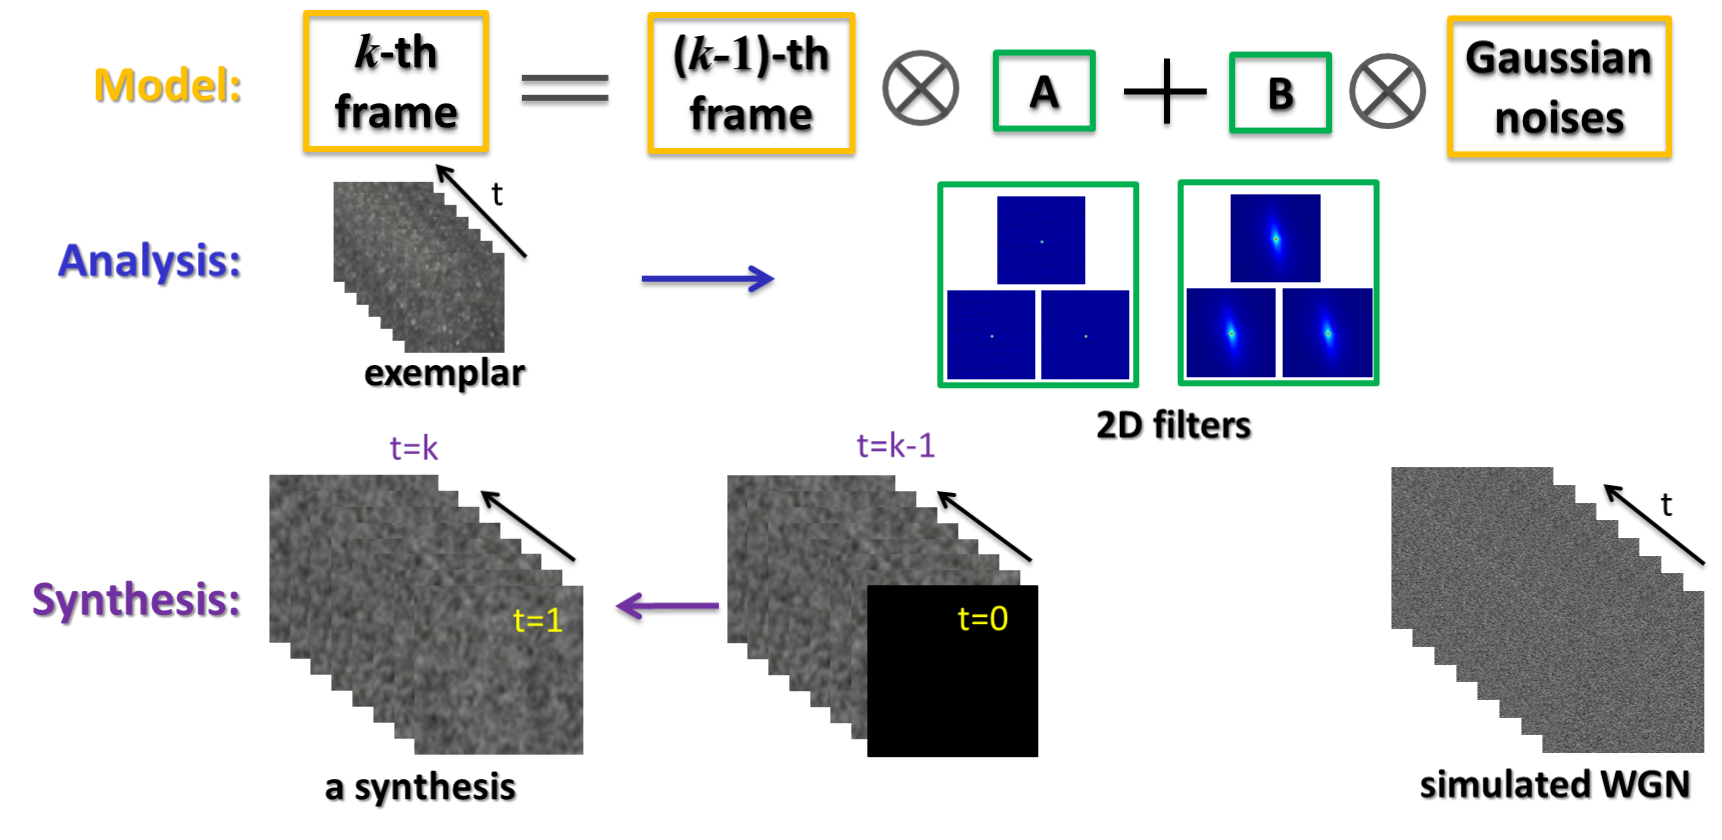
\includegraphics[width=0.9 \linewidth]{ar-model.png}
%  \caption{AR-texton for texture modeling. Observe that the parameters $(a,b)$ are in fact 2D filters. The analysis is to learn the 2D filters, and the synthesis is to modulate the input white Gaussian noise with the learned 2D filters. The first frame of the synthesized can be initialized randomly or by zeros, as the AR process converges quickly. }
%  \label{fig:ar-texton-synthesis}
%\end{figure}


%%%%%%%%%%%%%%%%%%%%%%%%%%%%%%%%%%%%%%%%%%%%%%%%%%%%%%%%%%%%%%%
\subsection{AR-Texton} 

The SVD decomposition of $\hat B(\om)$ reads
\eq{
	\foralls \om, \quad 
	\hat B(\om) = 
	\hat V(\om) \diag( \rho_1(\om),\ldots,\rho_d(\om) )  \hat V(\om)^* \in \CC^{d \times d}
}
%SIRA U already used for the domain, and it is used too close, I change to V:	\hat U(\om) \diag( \rho_1(\om),\ldots,\rho_d(\om) )  \hat U(\om)^* \in \CC^{d \times d}


where $(\rho_1(\om),\ldots,\rho_d(\om)) \in \RR_+^d$ are the eigenvalues of $\hat B(\om)$, and $\hat V(\om) \in \CC^{d \times d}$ is the unitary matrix of eigenvectors.

We denote by $\textonAR$ the canonical texton (compare to \eqref{eq-svd-canonical-texton} for the SN case) associated to $\Bb$
\eql{\label{eq-texton-AR-fourier-generic}
	\hat \textonAR(\om) = \hat V(\om)  \diag( \rho_1(\om)^{1/2},\ldots,\rho_d(\om)^{1/2} )\hat V(\om)^* \in \CC^{d \times d}
}
%SIRA U already used for the domain, and it is used too close, I change to V:	\hat \textonAR(\om) = \hat U(\om)  \diag( \rho_1(\om)^{1/2},\ldots,\rho_d(\om)^{1/2} )\hat U(\om)^* \in \CC^{d \times d}
We call the pair $(\Aa,\TextonAR)$ the AR-texton associated to the AR model.

%%%%%%%%%%%%%%%%%%%%%%%%%%%%%%%%%%%%%%%%%%%%%%%%%%%%%%%%%%%%%%%
\subsection{Resizing}

The texton $(\Aa,\TextonAR)$ can be resized to any new spatial domain $\tilde \Ux = \{0,\ldots,\tilde N_1 \} \times \{0,\ldots,\tilde N_2 -1 \}$ by cropping/zero-padding the initial kernels $(A,\textonAR)$ into $(\tilde \Aa, \tilde \TextonAR)$
%One can manipulate the textons $(\Aa,\TextonAR)$ to resize the model to any given output spacial domain $\tilde \Ux = \{0,\ldots,\tilde N_1 \} \times \{0,\ldots,\tilde N_2 -1 \}$. One computes $(\tilde \Aa, \tilde \TextonAR)$ by cropping/zero padding the initial kernels $(A,\textonAR)$
\eql{\label{eq-model-resize-AR}
	\foralls x \in \tilde \Ux, \quad
	\tilde  A(x) = 
	\choice{
		A(x) \qifq p \in \Ux, \\
		0 \quad \text{otherwise},
	}
}
(and similarly for $\TextonAR$).

%%%%%%%%%%%%%%%%%%%%%%%%%%%%%%%%%%%%%%%%%%%%%%%%%%%%%%%%%%%%%%%
\subsection{Texture Synthesis} 

Once the texton $(\tilde\Aa,\tilde\TextonAR)$ has been learned, a texture $f$ is obtained by sampling the model \eqref{eq-AR-stationary} from an initial time $t_0$
\eql{\label{eq-sample-ar}
	\foralls t \geq t_0, \quad 
	f_{t+1} = A \star f_t + \textonAR \star w_t
	\qwhereq 
	w_t \SampledFrom \Nn(0,\Id_{\Ux \times d}	)
}
where $f_{t_0}$ is drawn from any distribution (for instance $f_{t_0}=0$).

%A difficulty is that one needs to initialize the sampling at some initial time $t_0$ and that the 
We should note that a resulting texture is sampled from a time-stationary process only in the limit $t_0 \rightarrow -\infty$. In practice, only a few time steps $t_0 \leq t < 0$ are needed to reach almost stationarity. We thus initialize the sampling at some initial time $t_0$, we generate $\tilde N_3+t_0$ frames,  and we then discard the first $t_0$ samples, and we  consider $f = (f_{t})_{t=0}^{\tilde N_3-1}$ where $\tilde N_3$ is the number of desired frames. 
